% Chapter 5

\chapter{The pairing and the chemical potentials} % Main chapter title

\label{Chapter5} % For referencing the chapter elsewhere, use \ref{Chapter3} 

\lhead{Chapter 5. \emph{Pairing and chemical potentials}} % This is for the header on each page - perhaps a shortened title

%----------------------------------------------------------------------------------------
In this chapter we will first derive an integral equation for the chemical and pairing potentials; the socalled gap equation. This is done in section \ref{sec.pairingpotential.integralequation}. Fundamentally the interaction of the fermions will alter the chemical potential from the one for the free gas. For this reason we summarize some properties of the chemical potential for a free fermion gas in one dimension. This is done in section \ref{sec.chemicalpotential.freegas}. Using the number equation we then derive a second integral equation containing the chemical potential and the pairing. See section \ref{sec.chemicalpotential.numberequation}. In this way we are finally able to solve for both simultaneously. This is done numerically in section \ref{sec.pairingandchemicalpotential.numericalcalculation}.

\section{The gap equation} \label{sec.pairingpotential.integralequation}
In this section we find an integral equation for the pairing potential $\Delta_k$, known as the gap equation. Inspecting the definition in equation \eqref{eq.pairingpotentialdef} we see, that we need to calculate $\langle f_k f_{-k} \rangle$, which in turn specifies another term in the Hamiltonian: $\langle f^\dagger_k f^\dagger_{-k} \rangle$. From the transformation defined in equation \eqref{eq.fermionquasiparticledef}, we get that $f_k = u^*_{F,k}\zeta_k - v_{F,k}\zeta^\dagger_{-k}$ and $f_{-k} = v_{F,k}\zeta^\dagger_k + u^*_{F,k}\zeta_{-k}$. Hereby:
\begin{align}
\langle f_k f_{-k} \rangle &= \left \langle (u^*_{F,k}\zeta_k - v_{F,k}\zeta^\dagger_{-k}) (v_{F,k}\zeta^\dagger_k + u^*_{F,k}\zeta_{-k}) \right \rangle = u^*_{F,k}v_{F,k}\left[ \left \langle \zeta_k \zeta^\dagger_{k} \right \rangle - \left \langle \zeta^\dagger_{-k} \zeta_{-k} \right \rangle \right]  \nonumber \\
& =  u^*_{F,k}v_{F,k}\left[ 1 - \left \langle \zeta^\dagger_{k} \zeta_k \right \rangle - \left \langle \zeta^\dagger_{-k} \zeta_{-k} \right \rangle \right] = u^*_{F,k}v_{F,k}\left[1 - 2f(E_{F,k})\right], \nonumber
\end{align}
where we in the last equality use, that $\left \langle \zeta^\dagger_{k} \zeta_{k} \right \rangle = f(E_{F,k})=(\exp(\beta E_{F,k})+1)^{-1} $. Inserting this into the expression for $\Delta_k$ and using the relation $\frac{v_{F,k}\Delta^*_k}{u_{F,k}}=E_{F,k}-\varepsilon_k$ from equation \eqref{eq.Kitaev.uk_vk} we get the gap equation on as a sum:
\begin{equation}
\Delta_k = - \frac{1}{\mathcal{L}}\sum_{k'} W^\text{ind}_{FF}(k,k')\frac{\Delta_{k'}}{2E_{F,k'}}\tanh\left(\frac{\beta E_{F,k}}{2}\right).
\label{eq.GapequationSum}
\end{equation} 
As mentioned in the start of chapter \ref{Chapter2}, we use periodic boundary conditions of the string to investigate the bulk properties. This means, that the spacing of the $k$-points are $dk = \frac{2\pi}{\mathcal{L}}$, and so we can transform the above into the following integral:
\begin{equation}
\Delta_k = - \int \frac{dk'}{2\pi} W^\text{ind}_{FF}(k,k')\frac{\Delta_{k'}}{2E_{F,k'}}\tanh\left(\frac{\beta E_{F,k}}{2}\right), 
\label{eq.GapequationIntegral}
\end{equation} 
and hereby canceling the length $\mathcal{L}$. Because of the symmetries of the coupling potential summarized in equation \eqref{eq.CouplingPotentialSymmetries}, we see, that $W^\text{ind}_{FF}(0,k') = 0$. Hence, it is immediately clear from both equation \eqref{eq.GapequationSum} and \eqref{eq.GapequationIntegral}, that $\Delta_{k=0} = 0$ for any temperature. This means, that $E_{F,k=0} = |\mu| > 0$. Further it must then be the case that $k_c = \min_k \frac{E_{F,k}}{|k|} > 0$, and so the Landau condition for superfluidity is fulfilled\cite{LandauStatPhys2,PlischkeStatPhys}.
Specifically Landau has argued, that if this minimum $k_c$ does not occur at $k=0$, then quasiparticles propagating with $|k|< k_c$ will do so without friction. We can therefore already see, that the one dimensional string will be a superfluid for lowlying $k$-states. The exact value of $k_c$ requires a further analysis. 

Written out in the $l_t \to 0$ limit and with unitless quantities denoted by tildes, the gap integral is:
\begin{equation}
\tilde{\Delta}_{\tilde{k}} = \frac{2}{\pi^3}\frac{n_B}{n_F^3}(k_Fa_{BF})^2\left(\frac{m_F}{m_B} + \frac{m_B}{m_F}+ 2\right) \int_0^\infty d\tilde{k}' \; \ln\left[\frac{(\tilde{k}+\tilde{k}')^2+2/\tilde{\xi}^2}{(\tilde{k}-\tilde{k}')^2+2/\tilde{\xi}^2}\right] \frac{\tilde{\Delta}_{\tilde{k}'}}{\tilde{E}_{F,\tilde{k}'}}\tanh\left[\frac{\tilde{E}_{F,k}}{2\tilde{T}}\right],
\label{eq.GapequationIntegralUnitless}
\end{equation} 
where $\tilde{\xi} = k_F\xi = \frac{\pi}{\sqrt{8 n_B/n_F^3 k_Fa_B}}$, and $\tilde{E}_{F,\tilde{k}} = \sqrt{(\tilde{k}^2-\tilde{\mu})^2 + |\tilde{\Delta}_{\tilde{k}}|^2}$. We have also made use of the fact, that the integrand is even i $\tilde{k}'$. Notice, that since we are neglecting retardation effects, we assume $\left(\frac{m_F}{m_B}\right)^2\frac{4}{\pi^2}\frac{n_B}{n_F^3}k_Fa_B \gg 1$ as discussed in section \ref{sec.RetardationEffects}. If the stronger condition, that $\frac{n_B}{n_F^3}k_Fa_B \gg 1$ is fullfilled, we see that we are only investigating short ranged interactions between the fermions, since $k_F\xi \ll 1$ in this limit. 

\section{The number equation} \label{sec.chemicalpotential.numberequation}
In this section we use the number equation to derive a second integral equation for the chemical and pairing potentials. The number equation is: $N_F = \sum_k \left \langle f_k^\dagger f_k \right \rangle$, where we average with respect to the thermalized state of the system. From earlier we know, that $f_k = u_{F,k}^* \zeta_k -v_{F,k} \zeta_{-k}^\dagger$. This leads to the sum formula:
\begin{equation}
N_F = \sum_k \left(|u_{F,k}|^2-|v_{F,k}|^2\right) f(E_{F,k}) + |v_{F,k}|^2,\nonumber
\end{equation}
where $f(E_{F,k}) = (\exp(\beta E_{F,k}) + 1)^{-1}$ is the distribution of the fermion quasiparticles. Using the expression for the $u$ and $v$ coefficients, we get:
\begin{equation}
n_F = \int \frac{dk}{2\pi} \frac{\varepsilon_k}{E_{F,k}}f(E_{F,k}) + \frac{1}{2}\left(1 - \frac{\varepsilon_k}{E_{F,k}}\right), \nonumber
\end{equation}
where $n_F = N_F/\mathcal{L}$. For the free fermion gas $k_F = n_{F,0}\pi$. Since we consider $N_F$ and $\mathcal{L}$ as constant $n_F = n_{F,0}$. By going to unitless quantities, we hereby obtain:
\begin{equation}
1 = \int_0^\infty d\tilde{k} \; \frac{\tilde{\varepsilon}_{\tilde{k}}}{\tilde{E}_{F,k}}\frac{1}{\text{e}^{ \tilde{E}_{F,\tilde{k}}/\tilde{T} } + 1 } + \frac{1}{2}\left(1 - \frac{\tilde{\varepsilon}_{\tilde{k}}}{\tilde{E}_{F,\tilde{k}}}\right). 
\label{eq.NumberEquationUnitless}
\end{equation}
This gives us the required second equation.

\section{Assumptions}
Before performing the numerical calculation, it is worthwhile to summarize what assumptions, we have made so far. To trap the fermions in one dimension we assumed, that the transverse energy, $\omega_t$, is much larger than the typical energy of the fermions, $\epsilon_{F,0}$. This lead to requirement in the first line of table \ref{tab.assumptions}. To have neglible ground state depletion of the condensate, we saw in equation \eqref{eq.excitedbosonsBEC}, that we needed to assume $(n_Ba_B^3)^{1/3}\ll 1$. This is line two of the table. Further, to be able to neglect retardation effects, we needed to assume, that the fermions moves slowly relative to the quasiparticles in the BEC. This lead to the requirement in line 3 in the table.

\begin{table}[htb]
\centering
\caption{\textit{Summary of the assumptions made so far. $m_r = \frac{m_Fm_B}{m_F+m_B}$ is the reduced mass. B and F refer to Bosons and Fermions respectively. $\omega_n$ is the bosonic Matsubara frequencies associated with the induced interaction.}}
\begin{tabular}{|l|l|r|l|}
\hline \textbf{Quantity} & \textbf{Parameters} 				& \textbf{Assumption}						& \textbf{Reason}	\\
\hline Transverse energy gap & $\omega_t = 1/\sqrt{m_Fl_t}$ & $(k_Fl_t)^2/2 	\ll 1$ 					& Trap in transverse ground state \\
\hline B-B scattering length & $g_B = 4\pi a_B/m_B$			& $(n_Ba_B^3)^{1/3}	\ll 1$					& Negligible BEC depletion  \\
\hline $\omega_n = 0$ limit  & $n_B, a_B, m_F, m_B$			& $(\frac{m_F}{m_B})^2 \frac{n_B}{n_F^3}k_Fa_B \gg 1$ & Negligible retardation effects  \\
\hline B-F scattering length & $g_{BF} = 2\pi a_{BF}/m_r$ 	& $(n_Ba_{BF}^3)^{1/3}	\ll 1$				& Simple diagrammatics\\
\hline 
\end{tabular}
\label{tab.assumptions}
\end{table}

\section{Calculating the pairing potential} \label{sec.pairingandchemicalpotential.numericalcalculation}
In this section we will describe and perform a numerical calculation of the pairing and chemical potentials. The numerical calculation is based on the following idea. We start at $T=0$ and make an initial guess for $\Delta_k$ and $\mu(T=0)$. Then we plug this into the gap equation \eqref{eq.GapequationIntegralUnitless} for $\beta = 1/k_BT = \infty$ and hereby obtain a better result for $\Delta_k(T=0)$. This is then inserted into the number equation \eqref{eq.NumberEquationUnitless}, whereby we get an updated guess for the chemical potential. The process is repeated until the maximum of $\Delta_k(T=0)$ \textit{and} the Fermi energy $\mu(T=0)$ does not change by more than $1\%$. Afterwards we increase the temperature with a small increment $dT$ and use $\Delta_k(T=0)$ and $\mu(T=0$ as an initial guesses repeating the process for $T=0$. This is done for rising temperatures until we reach some critial temperature, where $\Delta_k(T_c)\approx 0$ for all $k$, somewhat equivalent to the original BCS-theory\cite{Tinkham,LandauStatPhys2,PlischkeStatPhys}. The procedure is quite slow, because we need the entire function $\Delta_k$ for each $k$-value in the iteration. Finally, we will use the $l_t \to 0$ limit for the coupling potential from equation \eqref{eq.CouplingPotentiallt=0} and so the gap equation of interest is equation \eqref{eq.GapequationIntegralUnitless}. It is possible to come with some rather well educated initial guesses for the pairing and the chemical potentials. We expect, that the chemical potential is not altered significantly from the one for the free gas, and so $\tilde{\mu}(T = 0) = 1$ is a good initial guess. The pairing needs to be odd in $k$ and by inspecting the integral equation, we see that we only get significant contributions around $\tilde{k}' = \tilde{k}$. Hence, we expect that the pairing goes to 0 for large values of $\tilde{k}$.  

The iteration over the pairing and chemical potentials are halted, when $\max_k[\Delta_k]$ and $\mu(T)$ do not change more than $1$\textperthousand upon iteration. An increasing number of iterations are needed near the transition from the superconducting to normal phase. Near the transition temperature $T_C$ the maximal pairing has the asymptotic form:
\begin{equation}
\frac{\max_{k}[\Delta_k(T)]}{\epsilon_{F,0}} \approx \max_k[\Delta_{k}(T=0)]\frac{T}{T_F}\left[1 - \left(\frac{T}{T_C}\right)^3\right]^{1/2}. 
\label{eq.maxpairingasymp}
\end{equation}
This resembles the original BCS-theory apart from the power of 3 of $\frac{T}{T_C}$. Near $T_C = 0.252 T_{F,0}$ the numerical calculation needs an increasing number of iterations. We therefore halt the calculation above $T_C$ and set $\Delta_k = 0$ for all $k$. This leads to the figures \ref{fig.Deltakkdepend} and \ref{fig.maxkDeltakTdepend}. From here we get, that $\max_{k,T}[\Delta_k(T)]/\epsilon_F \approx 0.562$. It follows, that the maximal gap to critical temperature ratio is: $\max_{k,T}[\Delta_k(T)]/(k_B T_C) \approx 2.23$. This is similar to the BCS-value of $1.77$ \cite{BruusFlensberg}.  

\begin{figure} 
\begin{center}  
% GNUPLOT: LaTeX picture with Postscript
\begingroup
  \makeatletter
  \providecommand\color[2][]{%
    \GenericError{(gnuplot) \space\space\space\@spaces}{%
      Package color not loaded in conjunction with
      terminal option `colourtext'%
    }{See the gnuplot documentation for explanation.%
    }{Either use 'blacktext' in gnuplot or load the package
      color.sty in LaTeX.}%
    \renewcommand\color[2][]{}%
  }%
  \providecommand\includegraphics[2][]{%
    \GenericError{(gnuplot) \space\space\space\@spaces}{%
      Package graphicx or graphics not loaded%
    }{See the gnuplot documentation for explanation.%
    }{The gnuplot epslatex terminal needs graphicx.sty or graphics.sty.}%
    \renewcommand\includegraphics[2][]{}%
  }%
  \providecommand\rotatebox[2]{#2}%
  \@ifundefined{ifGPcolor}{%
    \newif\ifGPcolor
    \GPcolorfalse
  }{}%
  \@ifundefined{ifGPblacktext}{%
    \newif\ifGPblacktext
    \GPblacktexttrue
  }{}%
  % define a \g@addto@macro without @ in the name:
  \let\gplgaddtomacro\g@addto@macro
  % define empty templates for all commands taking text:
  \gdef\gplbacktext{}%
  \gdef\gplfronttext{}%
  \makeatother
  \ifGPblacktext
    % no textcolor at all
    \def\colorrgb#1{}%
    \def\colorgray#1{}%
  \else
    % gray or color?
    \ifGPcolor
      \def\colorrgb#1{\color[rgb]{#1}}%
      \def\colorgray#1{\color[gray]{#1}}%
      \expandafter\def\csname LTw\endcsname{\color{white}}%
      \expandafter\def\csname LTb\endcsname{\color{black}}%
      \expandafter\def\csname LTa\endcsname{\color{black}}%
      \expandafter\def\csname LT0\endcsname{\color[rgb]{1,0,0}}%
      \expandafter\def\csname LT1\endcsname{\color[rgb]{0,1,0}}%
      \expandafter\def\csname LT2\endcsname{\color[rgb]{0,0,1}}%
      \expandafter\def\csname LT3\endcsname{\color[rgb]{1,0,1}}%
      \expandafter\def\csname LT4\endcsname{\color[rgb]{0,1,1}}%
      \expandafter\def\csname LT5\endcsname{\color[rgb]{1,1,0}}%
      \expandafter\def\csname LT6\endcsname{\color[rgb]{0,0,0}}%
      \expandafter\def\csname LT7\endcsname{\color[rgb]{1,0.3,0}}%
      \expandafter\def\csname LT8\endcsname{\color[rgb]{0.5,0.5,0.5}}%
    \else
      % gray
      \def\colorrgb#1{\color{black}}%
      \def\colorgray#1{\color[gray]{#1}}%
      \expandafter\def\csname LTw\endcsname{\color{white}}%
      \expandafter\def\csname LTb\endcsname{\color{black}}%
      \expandafter\def\csname LTa\endcsname{\color{black}}%
      \expandafter\def\csname LT0\endcsname{\color{black}}%
      \expandafter\def\csname LT1\endcsname{\color{black}}%
      \expandafter\def\csname LT2\endcsname{\color{black}}%
      \expandafter\def\csname LT3\endcsname{\color{black}}%
      \expandafter\def\csname LT4\endcsname{\color{black}}%
      \expandafter\def\csname LT5\endcsname{\color{black}}%
      \expandafter\def\csname LT6\endcsname{\color{black}}%
      \expandafter\def\csname LT7\endcsname{\color{black}}%
      \expandafter\def\csname LT8\endcsname{\color{black}}%
    \fi
  \fi
    \setlength{\unitlength}{0.0500bp}%
    \ifx\gptboxheight\undefined%
      \newlength{\gptboxheight}%
      \newlength{\gptboxwidth}%
      \newsavebox{\gptboxtext}%
    \fi%
    \setlength{\fboxrule}{0.5pt}%
    \setlength{\fboxsep}{1pt}%
\begin{picture}(7200.00,5040.00)%
    \gplgaddtomacro\gplbacktext{%
      \csname LTb\endcsname%
      \put(946,767){\makebox(0,0)[r]{\strut{}$-0.6$}}%
      \csname LTb\endcsname%
      \put(946,1468){\makebox(0,0)[r]{\strut{}$-0.4$}}%
      \csname LTb\endcsname%
      \put(946,2170){\makebox(0,0)[r]{\strut{}$-0.2$}}%
      \csname LTb\endcsname%
      \put(946,2871){\makebox(0,0)[r]{\strut{}$0$}}%
      \csname LTb\endcsname%
      \put(946,3573){\makebox(0,0)[r]{\strut{}$0.2$}}%
      \csname LTb\endcsname%
      \put(946,4275){\makebox(0,0)[r]{\strut{}$0.4$}}%
      \csname LTb\endcsname%
      \put(946,4976){\makebox(0,0)[r]{\strut{}$0.6$}}%
      \csname LTb\endcsname%
      \put(1141,484){\makebox(0,0){\strut{}$-10$}}%
      \csname LTb\endcsname%
      \put(2541,484){\makebox(0,0){\strut{}$-5$}}%
      \csname LTb\endcsname%
      \put(3941,484){\makebox(0,0){\strut{}$0$}}%
      \csname LTb\endcsname%
      \put(5340,484){\makebox(0,0){\strut{}$5$}}%
      \csname LTb\endcsname%
      \put(6740,484){\makebox(0,0){\strut{}$10$}}%
    }%
    \gplgaddtomacro\gplfronttext{%
      \csname LTb\endcsname%
      \put(176,2871){\rotatebox{-270}{\makebox(0,0){\strut{}$\Delta_k/\epsilon_{F,0}$}}}%
      \put(3940,154){\makebox(0,0){\strut{}$k/k_F$}}%
      \csname LTb\endcsname%
      \put(2725,4803){\makebox(0,0)[r]{\strut{}$T/T_F = 0.00$}}%
      \csname LTb\endcsname%
      \put(2725,4583){\makebox(0,0)[r]{\strut{}$T/T_F = 0.15$}}%
      \csname LTb\endcsname%
      \put(2725,4363){\makebox(0,0)[r]{\strut{}$T/T_F = 0.20$}}%
      \csname LTb\endcsname%
      \put(2725,4143){\makebox(0,0)[r]{\strut{}$T/T_F = 0.24$}}%
      \csname LTb\endcsname%
      \put(2725,3923){\makebox(0,0)[r]{\strut{}$T/T_F = 0.25$}}%
    }%
    \gplbacktext
    \put(0,0){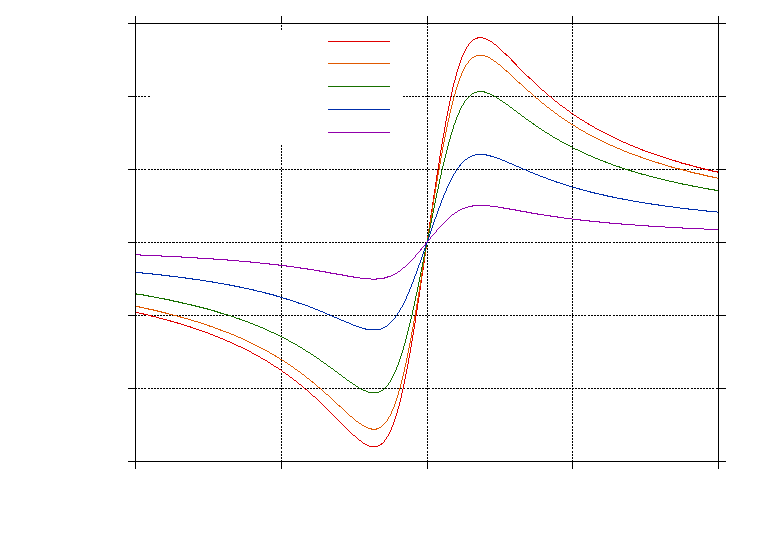
\includegraphics{Figures/Delta4/kdepend}}%
    \gplfronttext
  \end{picture}%
\endgroup
  
\caption{The numerically calculated gap $\Delta_k$ is plotted as a function of $k$ for different temperatures. Parameters: $(n_Ba_B^3)^{1/3} = 0.01, (n_Ba_B^3)^{1/3} = 0.04, l_t = 0, \frac{m_B}{m_F} = 7/40, \frac{n_F}{n_B^{1/3}} = 0.215, (m_F/m_B)^2n_B/n_F^3 kFaB = 22.10$. }  
\label{fig.Deltakkdepend}  
\end{center}    
\end{figure}

\begin{figure} 
\begin{center}  
% GNUPLOT: LaTeX picture with Postscript
\begingroup
  \makeatletter
  \providecommand\color[2][]{%
    \GenericError{(gnuplot) \space\space\space\@spaces}{%
      Package color not loaded in conjunction with
      terminal option `colourtext'%
    }{See the gnuplot documentation for explanation.%
    }{Either use 'blacktext' in gnuplot or load the package
      color.sty in LaTeX.}%
    \renewcommand\color[2][]{}%
  }%
  \providecommand\includegraphics[2][]{%
    \GenericError{(gnuplot) \space\space\space\@spaces}{%
      Package graphicx or graphics not loaded%
    }{See the gnuplot documentation for explanation.%
    }{The gnuplot epslatex terminal needs graphicx.sty or graphics.sty.}%
    \renewcommand\includegraphics[2][]{}%
  }%
  \providecommand\rotatebox[2]{#2}%
  \@ifundefined{ifGPcolor}{%
    \newif\ifGPcolor
    \GPcolorfalse
  }{}%
  \@ifundefined{ifGPblacktext}{%
    \newif\ifGPblacktext
    \GPblacktexttrue
  }{}%
  % define a \g@addto@macro without @ in the name:
  \let\gplgaddtomacro\g@addto@macro
  % define empty templates for all commands taking text:
  \gdef\gplbacktext{}%
  \gdef\gplfronttext{}%
  \makeatother
  \ifGPblacktext
    % no textcolor at all
    \def\colorrgb#1{}%
    \def\colorgray#1{}%
  \else
    % gray or color?
    \ifGPcolor
      \def\colorrgb#1{\color[rgb]{#1}}%
      \def\colorgray#1{\color[gray]{#1}}%
      \expandafter\def\csname LTw\endcsname{\color{white}}%
      \expandafter\def\csname LTb\endcsname{\color{black}}%
      \expandafter\def\csname LTa\endcsname{\color{black}}%
      \expandafter\def\csname LT0\endcsname{\color[rgb]{1,0,0}}%
      \expandafter\def\csname LT1\endcsname{\color[rgb]{0,1,0}}%
      \expandafter\def\csname LT2\endcsname{\color[rgb]{0,0,1}}%
      \expandafter\def\csname LT3\endcsname{\color[rgb]{1,0,1}}%
      \expandafter\def\csname LT4\endcsname{\color[rgb]{0,1,1}}%
      \expandafter\def\csname LT5\endcsname{\color[rgb]{1,1,0}}%
      \expandafter\def\csname LT6\endcsname{\color[rgb]{0,0,0}}%
      \expandafter\def\csname LT7\endcsname{\color[rgb]{1,0.3,0}}%
      \expandafter\def\csname LT8\endcsname{\color[rgb]{0.5,0.5,0.5}}%
    \else
      % gray
      \def\colorrgb#1{\color{black}}%
      \def\colorgray#1{\color[gray]{#1}}%
      \expandafter\def\csname LTw\endcsname{\color{white}}%
      \expandafter\def\csname LTb\endcsname{\color{black}}%
      \expandafter\def\csname LTa\endcsname{\color{black}}%
      \expandafter\def\csname LT0\endcsname{\color{black}}%
      \expandafter\def\csname LT1\endcsname{\color{black}}%
      \expandafter\def\csname LT2\endcsname{\color{black}}%
      \expandafter\def\csname LT3\endcsname{\color{black}}%
      \expandafter\def\csname LT4\endcsname{\color{black}}%
      \expandafter\def\csname LT5\endcsname{\color{black}}%
      \expandafter\def\csname LT6\endcsname{\color{black}}%
      \expandafter\def\csname LT7\endcsname{\color{black}}%
      \expandafter\def\csname LT8\endcsname{\color{black}}%
    \fi
  \fi
    \setlength{\unitlength}{0.0500bp}%
    \ifx\gptboxheight\undefined%
      \newlength{\gptboxheight}%
      \newlength{\gptboxwidth}%
      \newsavebox{\gptboxtext}%
    \fi%
    \setlength{\fboxrule}{0.5pt}%
    \setlength{\fboxsep}{1pt}%
\begin{picture}(7200.00,5040.00)%
    \gplgaddtomacro\gplbacktext{%
      \csname LTb\endcsname%
      \put(946,767){\makebox(0,0)[r]{\strut{}$0$}}%
      \csname LTb\endcsname%
      \put(946,1469){\makebox(0,0)[r]{\strut{}$0.05$}}%
      \csname LTb\endcsname%
      \put(946,2170){\makebox(0,0)[r]{\strut{}$0.1$}}%
      \csname LTb\endcsname%
      \put(946,2872){\makebox(0,0)[r]{\strut{}$0.15$}}%
      \csname LTb\endcsname%
      \put(946,3573){\makebox(0,0)[r]{\strut{}$0.2$}}%
      \csname LTb\endcsname%
      \put(946,4275){\makebox(0,0)[r]{\strut{}$0.25$}}%
      \csname LTb\endcsname%
      \put(946,4976){\makebox(0,0)[r]{\strut{}$0.3$}}%
      \csname LTb\endcsname%
      \put(1141,484){\makebox(0,0){\strut{}$0$}}%
      \csname LTb\endcsname%
      \put(1888,484){\makebox(0,0){\strut{}$0.02$}}%
      \csname LTb\endcsname%
      \put(2634,484){\makebox(0,0){\strut{}$0.04$}}%
      \csname LTb\endcsname%
      \put(3381,484){\makebox(0,0){\strut{}$0.06$}}%
      \csname LTb\endcsname%
      \put(4127,484){\makebox(0,0){\strut{}$0.08$}}%
      \csname LTb\endcsname%
      \put(4874,484){\makebox(0,0){\strut{}$0.1$}}%
      \csname LTb\endcsname%
      \put(5620,484){\makebox(0,0){\strut{}$0.12$}}%
      \csname LTb\endcsname%
      \put(6367,484){\makebox(0,0){\strut{}$0.14$}}%
    }%
    \gplgaddtomacro\gplfronttext{%
      \csname LTb\endcsname%
      \put(176,2871){\rotatebox{-270}{\makebox(0,0){\strut{}$\max_k[\Delta_k]/\epsilon_{F,0}$}}}%
      \put(3940,154){\makebox(0,0){\strut{}$T/T_F$}}%
    }%
    \gplbacktext
    \put(0,0){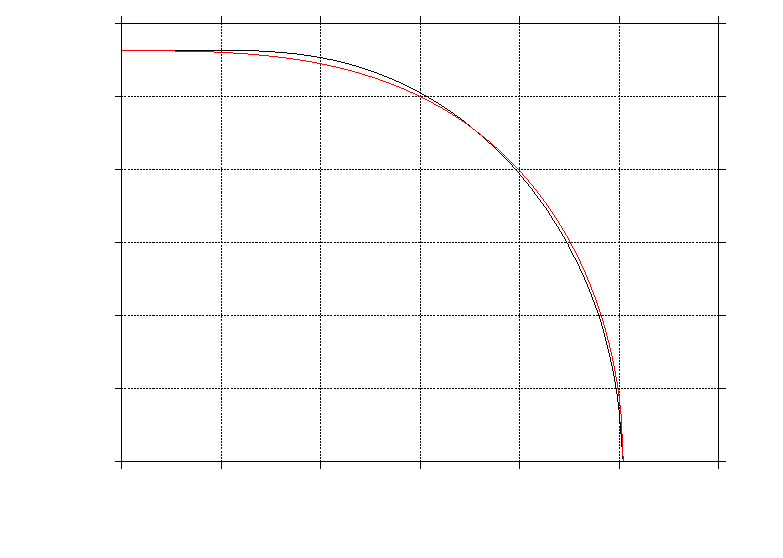
\includegraphics{Figures/Delta4/Tdepend}}%
    \gplfronttext
  \end{picture}%
\endgroup
  
\caption{In black: The numerically calculated maximal pairing $\max_k[\Delta_k]$. In red: the asymptotic form from equation \eqref{eq.maxpairingasymp}. This is seen to fit very well for both $T/T_C \ll 1$ and $T/T_C \approx 1$. Notice, that the critical temperature at which the pairing vanishes is $T_C \approx 0.150 T_{F,0}$, and that the gap is rapidly decreasing in the region $0.10< T/T_{F,0} < 0.15$. Parameters: $(n_Ba_B^3)^{1/3} = 0.01, (n_Ba_B^3)^{1/3} = 0.04, l_t = 0, \frac{m_B}{m_F} = 7/40, \frac{n_F}{n_B^{1/3}} = 0.215, (m_F/m_B)^2n_B/n_F^3 kFaB = 22.10$. }  
\label{fig.maxkDeltakTdepend}  
\end{center}    
\end{figure}

\begin{figure} 
\begin{center}  
% GNUPLOT: LaTeX picture with Postscript
\begingroup
  \makeatletter
  \providecommand\color[2][]{%
    \GenericError{(gnuplot) \space\space\space\@spaces}{%
      Package color not loaded in conjunction with
      terminal option `colourtext'%
    }{See the gnuplot documentation for explanation.%
    }{Either use 'blacktext' in gnuplot or load the package
      color.sty in LaTeX.}%
    \renewcommand\color[2][]{}%
  }%
  \providecommand\includegraphics[2][]{%
    \GenericError{(gnuplot) \space\space\space\@spaces}{%
      Package graphicx or graphics not loaded%
    }{See the gnuplot documentation for explanation.%
    }{The gnuplot epslatex terminal needs graphicx.sty or graphics.sty.}%
    \renewcommand\includegraphics[2][]{}%
  }%
  \providecommand\rotatebox[2]{#2}%
  \@ifundefined{ifGPcolor}{%
    \newif\ifGPcolor
    \GPcolortrue
  }{}%
  \@ifundefined{ifGPblacktext}{%
    \newif\ifGPblacktext
    \GPblacktexttrue
  }{}%
  % define a \g@addto@macro without @ in the name:
  \let\gplgaddtomacro\g@addto@macro
  % define empty templates for all commands taking text:
  \gdef\gplbacktext{}%
  \gdef\gplfronttext{}%
  \makeatother
  \ifGPblacktext
    % no textcolor at all
    \def\colorrgb#1{}%
    \def\colorgray#1{}%
  \else
    % gray or color?
    \ifGPcolor
      \def\colorrgb#1{\color[rgb]{#1}}%
      \def\colorgray#1{\color[gray]{#1}}%
      \expandafter\def\csname LTw\endcsname{\color{white}}%
      \expandafter\def\csname LTb\endcsname{\color{black}}%
      \expandafter\def\csname LTa\endcsname{\color{black}}%
      \expandafter\def\csname LT0\endcsname{\color[rgb]{1,0,0}}%
      \expandafter\def\csname LT1\endcsname{\color[rgb]{0,1,0}}%
      \expandafter\def\csname LT2\endcsname{\color[rgb]{0,0,1}}%
      \expandafter\def\csname LT3\endcsname{\color[rgb]{1,0,1}}%
      \expandafter\def\csname LT4\endcsname{\color[rgb]{0,1,1}}%
      \expandafter\def\csname LT5\endcsname{\color[rgb]{1,1,0}}%
      \expandafter\def\csname LT6\endcsname{\color[rgb]{0,0,0}}%
      \expandafter\def\csname LT7\endcsname{\color[rgb]{1,0.3,0}}%
      \expandafter\def\csname LT8\endcsname{\color[rgb]{0.5,0.5,0.5}}%
    \else
      % gray
      \def\colorrgb#1{\color{black}}%
      \def\colorgray#1{\color[gray]{#1}}%
      \expandafter\def\csname LTw\endcsname{\color{white}}%
      \expandafter\def\csname LTb\endcsname{\color{black}}%
      \expandafter\def\csname LTa\endcsname{\color{black}}%
      \expandafter\def\csname LT0\endcsname{\color{black}}%
      \expandafter\def\csname LT1\endcsname{\color{black}}%
      \expandafter\def\csname LT2\endcsname{\color{black}}%
      \expandafter\def\csname LT3\endcsname{\color{black}}%
      \expandafter\def\csname LT4\endcsname{\color{black}}%
      \expandafter\def\csname LT5\endcsname{\color{black}}%
      \expandafter\def\csname LT6\endcsname{\color{black}}%
      \expandafter\def\csname LT7\endcsname{\color{black}}%
      \expandafter\def\csname LT8\endcsname{\color{black}}%
    \fi
  \fi
    \setlength{\unitlength}{0.0500bp}%
    \ifx\gptboxheight\undefined%
      \newlength{\gptboxheight}%
      \newlength{\gptboxwidth}%
      \newsavebox{\gptboxtext}%
    \fi%
    \setlength{\fboxrule}{0.5pt}%
    \setlength{\fboxsep}{1pt}%
\begin{picture}(7200.00,5040.00)%
    \gplgaddtomacro\gplbacktext{%
      \csname LTb\endcsname%
      \put(814,767){\makebox(0,0)[r]{\strut{}$0$}}%
      \csname LTb\endcsname%
      \put(814,1532){\makebox(0,0)[r]{\strut{}$0.2$}}%
      \csname LTb\endcsname%
      \put(814,2298){\makebox(0,0)[r]{\strut{}$0.4$}}%
      \csname LTb\endcsname%
      \put(814,3063){\makebox(0,0)[r]{\strut{}$0.6$}}%
      \csname LTb\endcsname%
      \put(814,3828){\makebox(0,0)[r]{\strut{}$0.8$}}%
      \csname LTb\endcsname%
      \put(814,4593){\makebox(0,0)[r]{\strut{}$1$}}%
      \csname LTb\endcsname%
      \put(1009,484){\makebox(0,0){\strut{}$0$}}%
      \csname LTb\endcsname%
      \put(2442,484){\makebox(0,0){\strut{}$0.5$}}%
      \csname LTb\endcsname%
      \put(3875,484){\makebox(0,0){\strut{}$1$}}%
      \csname LTb\endcsname%
      \put(5307,484){\makebox(0,0){\strut{}$1.5$}}%
      \csname LTb\endcsname%
      \put(6740,484){\makebox(0,0){\strut{}$2$}}%
    }%
    \gplgaddtomacro\gplfronttext{%
      \csname LTb\endcsname%
      \put(176,2871){\rotatebox{-270}{\makebox(0,0){\strut{}$\braket{c_k^\dagger c_k}$}}}%
      \put(3874,154){\makebox(0,0){\strut{}$k/k_F$}}%
      \csname LTb\endcsname%
      \put(5753,4803){\makebox(0,0)[r]{\strut{}Free gas}}%
      \csname LTb\endcsname%
      \put(5753,4583){\makebox(0,0)[r]{\strut{}$r_B = 0.005$}}%
      \csname LTb\endcsname%
      \put(5753,4363){\makebox(0,0)[r]{\strut{}$r_B = 0.006$}}%
      \csname LTb\endcsname%
      \put(5753,4143){\makebox(0,0)[r]{\strut{}$r_B = 0.007$}}%
      \csname LTb\endcsname%
      \put(5753,3923){\makebox(0,0)[r]{\strut{}$r_B = 0.010$}}%
    }%
    \gplbacktext
    \put(0,0){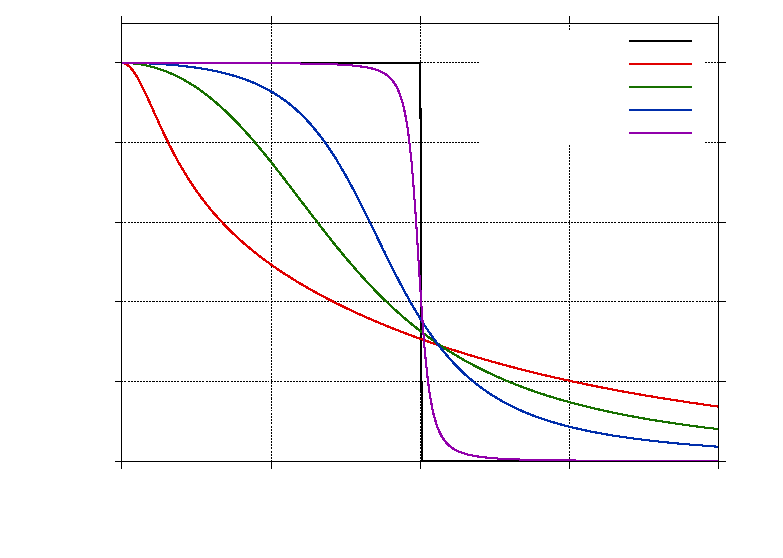
\includegraphics{Figures/OccupancyT0/Occupancyplot}}%
    \gplfronttext
  \end{picture}%
\endgroup
  
\caption{The number of fermions with momentum $k$, $\braket{f_k^\dagger f_k}$, is plotted as a function of $k$ for $T = 0$. $\braket{f_k^\dagger f_k} = |v_{F,k}|^2 = \frac{1}{2}\left(1 - \frac{\epsilon_k}{E_{F,k}}\right)$. Since $E_{F,k} = \sqrt{\epsilon_k^2 + |\Delta_k|^2}$ we recover the Fermi-Dirac distribution for the free gas, when $\Delta_k = 0$. This is shown in black. The colored lines are for the superconducting string for different values of the Bose gas parameter $r_B = (n_Ba_B^3)^{1/3}$.  }  
\label{fig.Occupancy}  
\end{center}    
\end{figure}

 We observe for the solution at hand, that the pairing potential is uneven in $k$ as already argued, and that it goes to 0 for $k/k_F \gg 1$. This decay does not seem to be exponential, but rather of a power type. Further, the maximum value of the gap $\max_k[\Delta_k]$ decreases monotonically to 0 in a similar manner to the original BCS-theory. See \cite{Tinkham,BruusFlensberg,PlischkeStatPhys} for details. Finally, the chemical potential has not been plotted. Since the chemical potential numerically changes very little from the free gas potential, a very high resolution in $k$ is needed to get an accurate numerical result. Therefore, we do not plot the chemical potential and instead use the number equation only to enhance the precision of the found pairing. We do however see, that the chemical potential is shifted downwards for $T=0$. This is physically reasonable, since it should cost less energy to add another fermion, when they are (partially) attracting each other through the induced interaction. Further, since the pairing goes continously to zero for $T\to T_C$ the chemical potential must go continuously to the free gas potential for $T\to T_C$. 

 We can enhance the pairing potential by decreasing the BEC scattering length $a_B$. This is connected to increasing the healing length $\tilde{\xi} = k_F\xi = \frac{\pi}{\sqrt{8 n_B/n_F^3 k_Fa_B}}$. In turn this is the range of the induced interaction in real space: $\tilde{V}_{FF}^\text{ind}(x,0) \propto \frac{\text{e}^{-\sqrt{2}|x|/\xi}}{|x|}$. The enhancement is thus physically reasonable. This behaviour is seen to match with the depicted in figure \ref{fig.maxkDeltakaBdepend}, and it shows, that there is a dramatic increase for $k_Fa_B \to +0$, or equivalently when the range $\xi$ of the induced interaction goes to infinity. Further, the pairing actually crosses the free gas Fermi energy. In the same analysis we find, that the Fermi energy $\epsilon_F$ is shifted about $6\%$ from the free gas Fermi energy $\epsilon_{F,0}$ for all values of $k_F a_B$.  

\begin{figure} 
\begin{center}  
% GNUPLOT: LaTeX picture with Postscript
\begingroup
  \makeatletter
  \providecommand\color[2][]{%
    \GenericError{(gnuplot) \space\space\space\@spaces}{%
      Package color not loaded in conjunction with
      terminal option `colourtext'%
    }{See the gnuplot documentation for explanation.%
    }{Either use 'blacktext' in gnuplot or load the package
      color.sty in LaTeX.}%
    \renewcommand\color[2][]{}%
  }%
  \providecommand\includegraphics[2][]{%
    \GenericError{(gnuplot) \space\space\space\@spaces}{%
      Package graphicx or graphics not loaded%
    }{See the gnuplot documentation for explanation.%
    }{The gnuplot epslatex terminal needs graphicx.sty or graphics.sty.}%
    \renewcommand\includegraphics[2][]{}%
  }%
  \providecommand\rotatebox[2]{#2}%
  \@ifundefined{ifGPcolor}{%
    \newif\ifGPcolor
    \GPcolorfalse
  }{}%
  \@ifundefined{ifGPblacktext}{%
    \newif\ifGPblacktext
    \GPblacktexttrue
  }{}%
  % define a \g@addto@macro without @ in the name:
  \let\gplgaddtomacro\g@addto@macro
  % define empty templates for all commands taking text:
  \gdef\gplbacktext{}%
  \gdef\gplfronttext{}%
  \makeatother
  \ifGPblacktext
    % no textcolor at all
    \def\colorrgb#1{}%
    \def\colorgray#1{}%
  \else
    % gray or color?
    \ifGPcolor
      \def\colorrgb#1{\color[rgb]{#1}}%
      \def\colorgray#1{\color[gray]{#1}}%
      \expandafter\def\csname LTw\endcsname{\color{white}}%
      \expandafter\def\csname LTb\endcsname{\color{black}}%
      \expandafter\def\csname LTa\endcsname{\color{black}}%
      \expandafter\def\csname LT0\endcsname{\color[rgb]{1,0,0}}%
      \expandafter\def\csname LT1\endcsname{\color[rgb]{0,1,0}}%
      \expandafter\def\csname LT2\endcsname{\color[rgb]{0,0,1}}%
      \expandafter\def\csname LT3\endcsname{\color[rgb]{1,0,1}}%
      \expandafter\def\csname LT4\endcsname{\color[rgb]{0,1,1}}%
      \expandafter\def\csname LT5\endcsname{\color[rgb]{1,1,0}}%
      \expandafter\def\csname LT6\endcsname{\color[rgb]{0,0,0}}%
      \expandafter\def\csname LT7\endcsname{\color[rgb]{1,0.3,0}}%
      \expandafter\def\csname LT8\endcsname{\color[rgb]{0.5,0.5,0.5}}%
    \else
      % gray
      \def\colorrgb#1{\color{black}}%
      \def\colorgray#1{\color[gray]{#1}}%
      \expandafter\def\csname LTw\endcsname{\color{white}}%
      \expandafter\def\csname LTb\endcsname{\color{black}}%
      \expandafter\def\csname LTa\endcsname{\color{black}}%
      \expandafter\def\csname LT0\endcsname{\color{black}}%
      \expandafter\def\csname LT1\endcsname{\color{black}}%
      \expandafter\def\csname LT2\endcsname{\color{black}}%
      \expandafter\def\csname LT3\endcsname{\color{black}}%
      \expandafter\def\csname LT4\endcsname{\color{black}}%
      \expandafter\def\csname LT5\endcsname{\color{black}}%
      \expandafter\def\csname LT6\endcsname{\color{black}}%
      \expandafter\def\csname LT7\endcsname{\color{black}}%
      \expandafter\def\csname LT8\endcsname{\color{black}}%
    \fi
  \fi
    \setlength{\unitlength}{0.0500bp}%
    \ifx\gptboxheight\undefined%
      \newlength{\gptboxheight}%
      \newlength{\gptboxwidth}%
      \newsavebox{\gptboxtext}%
    \fi%
    \setlength{\fboxrule}{0.5pt}%
    \setlength{\fboxsep}{1pt}%
\begin{picture}(7200.00,5040.00)%
    \gplgaddtomacro\gplbacktext{%
      \csname LTb\endcsname%
      \put(682,767){\makebox(0,0)[r]{\strut{}$0$}}%
      \csname LTb\endcsname%
      \put(682,1469){\makebox(0,0)[r]{\strut{}$5$}}%
      \csname LTb\endcsname%
      \put(682,2170){\makebox(0,0)[r]{\strut{}$10$}}%
      \csname LTb\endcsname%
      \put(682,2872){\makebox(0,0)[r]{\strut{}$15$}}%
      \csname LTb\endcsname%
      \put(682,3573){\makebox(0,0)[r]{\strut{}$20$}}%
      \csname LTb\endcsname%
      \put(682,4275){\makebox(0,0)[r]{\strut{}$25$}}%
      \csname LTb\endcsname%
      \put(682,4976){\makebox(0,0)[r]{\strut{}$30$}}%
      \csname LTb\endcsname%
      \put(877,484){\makebox(0,0){\strut{}$0$}}%
      \csname LTb\endcsname%
      \put(2050,484){\makebox(0,0){\strut{}$0.002$}}%
      \csname LTb\endcsname%
      \put(3222,484){\makebox(0,0){\strut{}$0.004$}}%
      \csname LTb\endcsname%
      \put(4395,484){\makebox(0,0){\strut{}$0.006$}}%
      \csname LTb\endcsname%
      \put(5567,484){\makebox(0,0){\strut{}$0.008$}}%
      \csname LTb\endcsname%
      \put(6740,484){\makebox(0,0){\strut{}$0.01$}}%
    }%
    \gplgaddtomacro\gplfronttext{%
      \csname LTb\endcsname%
      \put(176,2871){\rotatebox{-270}{\makebox(0,0){\strut{}$\max_{k}[\Delta_k(T=0)]/\epsilon_{F,0}$}}}%
      \put(3808,154){\makebox(0,0){\strut{}$(n_Ba_B^3)^{1/3}$}}%
    }%
    \gplbacktext
    \put(0,0){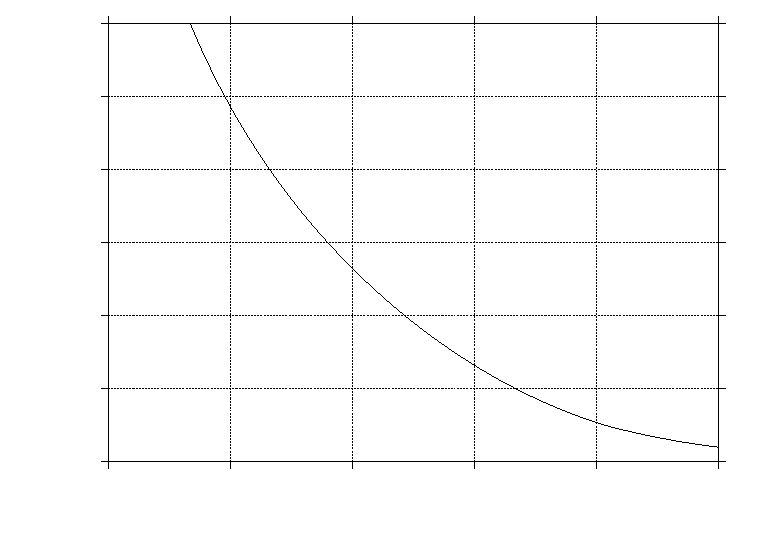
\includegraphics{Figures/DeltavaryrBB/rBBdepend}}%
    \gplfronttext
  \end{picture}%
\endgroup
  
\caption{The maximal pairing $\max_k[\Delta_k(T=0)]$ is plotted as a function of the BEC gas constant $(n_Ba_B^3)^{1/3}$. Notice the monotonic decrease. Other parameters: $(n_Ba_B^3)^{1/3} = 0.036, l_t = 0, \frac{m_B}{m_F} = 7/40, \frac{n_F}{n_B^{1/3}} = 0.036$.}  
\label{fig.maxkDeltakaBdepend}  
\end{center}    
\end{figure}


 We now turn our attention to the potential width for the string: $l_t$. Finding a solution for $l_t > 0$ is a little more tedious than for $l_t = 0$, since we then need to solve the integral for $V_{FF}^\text{ind}(q,0)$ for each iteration. It does however carry through analogously to the $l_t = 0$ case. Figure \ref{fig.maxkDeltakltdepend} shows the found dependency on $l_t$ of the maximal pairing. We see, that there is a well defined $l_t \to 0$ limit as expected, and that the maximal pairing decreases monotonically with $l_t$. This can best be understood again from the real space induced interaction. We saw in figure \ref{fig.Vx}, that the induced interaction is effectively shielded around $x = 0$ for $l_t > 0$. This shielding is increased for higher values of $l_t$. Hence, the interaction is lowered when the particles are close to each other. In conclusion the pairing most decrease with increasing $l_t$. 

\begin{figure} 
\begin{center}  
% GNUPLOT: LaTeX picture with Postscript
\begingroup
  \makeatletter
  \providecommand\color[2][]{%
    \GenericError{(gnuplot) \space\space\space\@spaces}{%
      Package color not loaded in conjunction with
      terminal option `colourtext'%
    }{See the gnuplot documentation for explanation.%
    }{Either use 'blacktext' in gnuplot or load the package
      color.sty in LaTeX.}%
    \renewcommand\color[2][]{}%
  }%
  \providecommand\includegraphics[2][]{%
    \GenericError{(gnuplot) \space\space\space\@spaces}{%
      Package graphicx or graphics not loaded%
    }{See the gnuplot documentation for explanation.%
    }{The gnuplot epslatex terminal needs graphicx.sty or graphics.sty.}%
    \renewcommand\includegraphics[2][]{}%
  }%
  \providecommand\rotatebox[2]{#2}%
  \@ifundefined{ifGPcolor}{%
    \newif\ifGPcolor
    \GPcolorfalse
  }{}%
  \@ifundefined{ifGPblacktext}{%
    \newif\ifGPblacktext
    \GPblacktexttrue
  }{}%
  % define a \g@addto@macro without @ in the name:
  \let\gplgaddtomacro\g@addto@macro
  % define empty templates for all commands taking text:
  \gdef\gplbacktext{}%
  \gdef\gplfronttext{}%
  \makeatother
  \ifGPblacktext
    % no textcolor at all
    \def\colorrgb#1{}%
    \def\colorgray#1{}%
  \else
    % gray or color?
    \ifGPcolor
      \def\colorrgb#1{\color[rgb]{#1}}%
      \def\colorgray#1{\color[gray]{#1}}%
      \expandafter\def\csname LTw\endcsname{\color{white}}%
      \expandafter\def\csname LTb\endcsname{\color{black}}%
      \expandafter\def\csname LTa\endcsname{\color{black}}%
      \expandafter\def\csname LT0\endcsname{\color[rgb]{1,0,0}}%
      \expandafter\def\csname LT1\endcsname{\color[rgb]{0,1,0}}%
      \expandafter\def\csname LT2\endcsname{\color[rgb]{0,0,1}}%
      \expandafter\def\csname LT3\endcsname{\color[rgb]{1,0,1}}%
      \expandafter\def\csname LT4\endcsname{\color[rgb]{0,1,1}}%
      \expandafter\def\csname LT5\endcsname{\color[rgb]{1,1,0}}%
      \expandafter\def\csname LT6\endcsname{\color[rgb]{0,0,0}}%
      \expandafter\def\csname LT7\endcsname{\color[rgb]{1,0.3,0}}%
      \expandafter\def\csname LT8\endcsname{\color[rgb]{0.5,0.5,0.5}}%
    \else
      % gray
      \def\colorrgb#1{\color{black}}%
      \def\colorgray#1{\color[gray]{#1}}%
      \expandafter\def\csname LTw\endcsname{\color{white}}%
      \expandafter\def\csname LTb\endcsname{\color{black}}%
      \expandafter\def\csname LTa\endcsname{\color{black}}%
      \expandafter\def\csname LT0\endcsname{\color{black}}%
      \expandafter\def\csname LT1\endcsname{\color{black}}%
      \expandafter\def\csname LT2\endcsname{\color{black}}%
      \expandafter\def\csname LT3\endcsname{\color{black}}%
      \expandafter\def\csname LT4\endcsname{\color{black}}%
      \expandafter\def\csname LT5\endcsname{\color{black}}%
      \expandafter\def\csname LT6\endcsname{\color{black}}%
      \expandafter\def\csname LT7\endcsname{\color{black}}%
      \expandafter\def\csname LT8\endcsname{\color{black}}%
    \fi
  \fi
    \setlength{\unitlength}{0.0500bp}%
    \ifx\gptboxheight\undefined%
      \newlength{\gptboxheight}%
      \newlength{\gptboxwidth}%
      \newsavebox{\gptboxtext}%
    \fi%
    \setlength{\fboxrule}{0.5pt}%
    \setlength{\fboxsep}{1pt}%
\begin{picture}(7200.00,5040.00)%
    \gplgaddtomacro\gplbacktext{%
      \csname LTb\endcsname%
      \put(946,767){\makebox(0,0)[r]{\strut{}$0$}}%
      \csname LTb\endcsname%
      \put(946,1446){\makebox(0,0)[r]{\strut{}$0.05$}}%
      \csname LTb\endcsname%
      \put(946,2125){\makebox(0,0)[r]{\strut{}$0.1$}}%
      \csname LTb\endcsname%
      \put(946,2804){\makebox(0,0)[r]{\strut{}$0.15$}}%
      \csname LTb\endcsname%
      \put(946,3482){\makebox(0,0)[r]{\strut{}$0.2$}}%
      \csname LTb\endcsname%
      \put(946,4161){\makebox(0,0)[r]{\strut{}$0.25$}}%
      \csname LTb\endcsname%
      \put(946,4840){\makebox(0,0)[r]{\strut{}$0.3$}}%
      \csname LTb\endcsname%
      \put(1141,484){\makebox(0,0){\strut{}$0$}}%
      \csname LTb\endcsname%
      \put(2074,484){\makebox(0,0){\strut{}$0.05$}}%
      \csname LTb\endcsname%
      \put(3007,484){\makebox(0,0){\strut{}$0.1$}}%
      \csname LTb\endcsname%
      \put(3941,484){\makebox(0,0){\strut{}$0.15$}}%
      \csname LTb\endcsname%
      \put(4874,484){\makebox(0,0){\strut{}$0.2$}}%
      \csname LTb\endcsname%
      \put(5807,484){\makebox(0,0){\strut{}$0.25$}}%
      \csname LTb\endcsname%
      \put(6740,484){\makebox(0,0){\strut{}$0.3$}}%
    }%
    \gplgaddtomacro\gplfronttext{%
      \csname LTb\endcsname%
      \put(176,2871){\rotatebox{-270}{\makebox(0,0){\strut{}$\max_{k}[\Delta_k(T=0)]/\epsilon_{F,0}$}}}%
      \put(3940,154){\makebox(0,0){\strut{}$k_Fl_t$}}%
    }%
    \gplbacktext
    \put(0,0){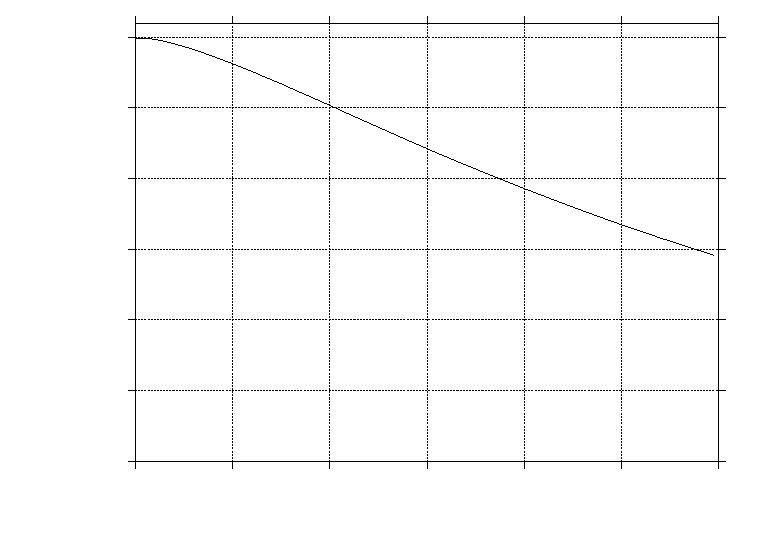
\includegraphics{Figures/Deltavarylt/ltdepend}}%
    \gplfronttext
  \end{picture}%
\endgroup
  
\caption{The maximal pairing $\max_k[\Delta_k(T=0)]$ is plotted as a function of the potential width $l_t$. Other parameters: $k_Fa_B = k_F a_{BF} = 0.3, \frac{m_B}{m_F} = 0.8, \frac{n_B}{n_F^3} = 1$.}  
\label{fig.maxkDeltakltdepend}  
\end{center}    
\end{figure}

Let us now investigate the dependency on the fermion-boson scattering length: $a_{BF}$. The result of the numerical calculation is shown in \ref{fig.maxkDeltakaBFdepend}. The pairing is seen to drop to zero around $k_Fa_{BF,c} = 0.155$. This shows, that the fermion-boson scattering length must exceed a cricital value for the string to be superconducting.   

\begin{figure} 
\begin{center}  
% GNUPLOT: LaTeX picture with Postscript
\begingroup
  \makeatletter
  \providecommand\color[2][]{%
    \GenericError{(gnuplot) \space\space\space\@spaces}{%
      Package color not loaded in conjunction with
      terminal option `colourtext'%
    }{See the gnuplot documentation for explanation.%
    }{Either use 'blacktext' in gnuplot or load the package
      color.sty in LaTeX.}%
    \renewcommand\color[2][]{}%
  }%
  \providecommand\includegraphics[2][]{%
    \GenericError{(gnuplot) \space\space\space\@spaces}{%
      Package graphicx or graphics not loaded%
    }{See the gnuplot documentation for explanation.%
    }{The gnuplot epslatex terminal needs graphicx.sty or graphics.sty.}%
    \renewcommand\includegraphics[2][]{}%
  }%
  \providecommand\rotatebox[2]{#2}%
  \@ifundefined{ifGPcolor}{%
    \newif\ifGPcolor
    \GPcolorfalse
  }{}%
  \@ifundefined{ifGPblacktext}{%
    \newif\ifGPblacktext
    \GPblacktexttrue
  }{}%
  % define a \g@addto@macro without @ in the name:
  \let\gplgaddtomacro\g@addto@macro
  % define empty templates for all commands taking text:
  \gdef\gplbacktext{}%
  \gdef\gplfronttext{}%
  \makeatother
  \ifGPblacktext
    % no textcolor at all
    \def\colorrgb#1{}%
    \def\colorgray#1{}%
  \else
    % gray or color?
    \ifGPcolor
      \def\colorrgb#1{\color[rgb]{#1}}%
      \def\colorgray#1{\color[gray]{#1}}%
      \expandafter\def\csname LTw\endcsname{\color{white}}%
      \expandafter\def\csname LTb\endcsname{\color{black}}%
      \expandafter\def\csname LTa\endcsname{\color{black}}%
      \expandafter\def\csname LT0\endcsname{\color[rgb]{1,0,0}}%
      \expandafter\def\csname LT1\endcsname{\color[rgb]{0,1,0}}%
      \expandafter\def\csname LT2\endcsname{\color[rgb]{0,0,1}}%
      \expandafter\def\csname LT3\endcsname{\color[rgb]{1,0,1}}%
      \expandafter\def\csname LT4\endcsname{\color[rgb]{0,1,1}}%
      \expandafter\def\csname LT5\endcsname{\color[rgb]{1,1,0}}%
      \expandafter\def\csname LT6\endcsname{\color[rgb]{0,0,0}}%
      \expandafter\def\csname LT7\endcsname{\color[rgb]{1,0.3,0}}%
      \expandafter\def\csname LT8\endcsname{\color[rgb]{0.5,0.5,0.5}}%
    \else
      % gray
      \def\colorrgb#1{\color{black}}%
      \def\colorgray#1{\color[gray]{#1}}%
      \expandafter\def\csname LTw\endcsname{\color{white}}%
      \expandafter\def\csname LTb\endcsname{\color{black}}%
      \expandafter\def\csname LTa\endcsname{\color{black}}%
      \expandafter\def\csname LT0\endcsname{\color{black}}%
      \expandafter\def\csname LT1\endcsname{\color{black}}%
      \expandafter\def\csname LT2\endcsname{\color{black}}%
      \expandafter\def\csname LT3\endcsname{\color{black}}%
      \expandafter\def\csname LT4\endcsname{\color{black}}%
      \expandafter\def\csname LT5\endcsname{\color{black}}%
      \expandafter\def\csname LT6\endcsname{\color{black}}%
      \expandafter\def\csname LT7\endcsname{\color{black}}%
      \expandafter\def\csname LT8\endcsname{\color{black}}%
    \fi
  \fi
    \setlength{\unitlength}{0.0500bp}%
    \ifx\gptboxheight\undefined%
      \newlength{\gptboxheight}%
      \newlength{\gptboxwidth}%
      \newsavebox{\gptboxtext}%
    \fi%
    \setlength{\fboxrule}{0.5pt}%
    \setlength{\fboxsep}{1pt}%
\begin{picture}(7200.00,5040.00)%
    \gplgaddtomacro\gplbacktext{%
      \csname LTb\endcsname%
      \put(550,767){\makebox(0,0)[r]{\strut{}$0$}}%
      \csname LTb\endcsname%
      \put(550,1368){\makebox(0,0)[r]{\strut{}$1$}}%
      \csname LTb\endcsname%
      \put(550,1970){\makebox(0,0)[r]{\strut{}$2$}}%
      \csname LTb\endcsname%
      \put(550,2571){\makebox(0,0)[r]{\strut{}$3$}}%
      \csname LTb\endcsname%
      \put(550,3172){\makebox(0,0)[r]{\strut{}$4$}}%
      \csname LTb\endcsname%
      \put(550,3773){\makebox(0,0)[r]{\strut{}$5$}}%
      \csname LTb\endcsname%
      \put(550,4375){\makebox(0,0)[r]{\strut{}$6$}}%
      \csname LTb\endcsname%
      \put(550,4976){\makebox(0,0)[r]{\strut{}$7$}}%
      \csname LTb\endcsname%
      \put(745,484){\makebox(0,0){\strut{}$0.03$}}%
      \csname LTb\endcsname%
      \put(1944,484){\makebox(0,0){\strut{}$0.032$}}%
      \csname LTb\endcsname%
      \put(3143,484){\makebox(0,0){\strut{}$0.034$}}%
      \csname LTb\endcsname%
      \put(4342,484){\makebox(0,0){\strut{}$0.036$}}%
      \csname LTb\endcsname%
      \put(5541,484){\makebox(0,0){\strut{}$0.038$}}%
      \csname LTb\endcsname%
      \put(6740,484){\makebox(0,0){\strut{}$0.04$}}%
    }%
    \gplgaddtomacro\gplfronttext{%
      \csname LTb\endcsname%
      \put(176,2871){\rotatebox{-270}{\makebox(0,0){\strut{}$\max_{k}[\Delta_k(T=0)]/\epsilon_{F,0}$}}}%
      \put(3742,154){\makebox(0,0){\strut{}$(n_Ba_{BF}^3)^{1/3}$}}%
    }%
    \gplbacktext
    \put(0,0){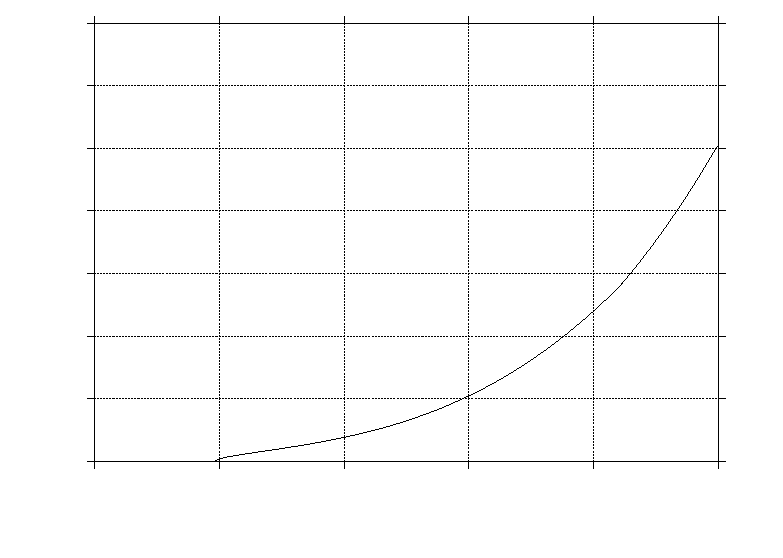
\includegraphics{Figures/DeltavaryrBF/rBFdepend}}%
    \gplfronttext
  \end{picture}%
\endgroup
  
\caption{The maximal pairing $\max_k[\Delta_k(T=0)]$ is plotted as a function of the fermion-boson gas constant $(n_Ba_{BF}^3)^{1/3}$. Notice that it goes rapidly to zero just below $(n_Ba_{BF}^3)^{1/3}= 0.032$. Other parameters: $l_t = 0, \frac{m_B}{m_F} = 7/40, \frac{n_F}{n_B^{1/3}} = 0.036$.}  
\label{fig.maxkDeltakaBFdepend}  
\end{center}    
\end{figure}

\section{The linearized gap equation} \label{sec.linearizedgapequation}
In the above analysis the estimation of the critical temperature $T_C$ is quite tedious. We have to wait for an increasing number of iterations near $T_C$ to get a good estimate and calculating the critical temperature as a function of the parameters of the problem is out of the question. In this section we will describe a much more efficient way of estimating the critical temperature through \textit{the linearized gap equation}. This in turn will be performed in section \ref{sec.pairingandchemicalpotential.numericalcalculation}, where the goal is to see the dependency of $T_C$ on the parameters of the system.

The gap equation in its full integral form is (see equation \eqref{eq.GapequationIntegral}):
\begin{equation}
\Delta_k = - \int \frac{dk'}{2\pi} W^\text{ind}_{FF}(k,k')\frac{\tanh\left(\frac{\beta E_{F,k}}{2}\right)}{2E_{F,k'}}\Delta_{k'}. \nonumber
\end{equation} 
As we saw explicitly in the previous section the gap goes to zero at the critical temperature $T_C$: $\Delta_k(T_C) = 0$. The energy $E_{F,k} = \sqrt{\epsilon_k^2 + |\Delta_k|^2}$ is quadratic in the gap. It follows that by only retaining the gap to first order, we obtain a linear equation near $T_C$:
\begin{equation}
\Delta_k = - \int \frac{dk'}{2\pi} W^\text{ind}_{FF}(k,k')\frac{\tanh\left(\frac{\beta \varepsilon_k}{2}\right)}{2\varepsilon_k} \Delta_{k'}.
\label{eq.GapequationIntegralLinear}
\end{equation} 
Here we have also used, that $\frac{\tanh\left(\frac{\beta \varepsilon_k}{2}\right)}{2\varepsilon_k}$ is even in $\varepsilon_k$, so that the absolute value stemming from the square root can be omitted. This defines a linear equation with eigenvalue $1$: $\Delta_k = L(\Delta_k)$. $L$ is then a linear transformation defined by the integral above. Hence, the program for the evaluation of $T_C$ is now clear. The eigenvalues of $L$ spans a continuum of values. Thus, to find $T_C$ we must find the temperature at which the largest eigenvalue becomes unity. 

\section{Calculating the critical temperature} \label{sec.pairingandchemicalpotential.numericalcalculation}
In this section we will describe how in practice to perform the calculation outlined in the above. 

To do the calculation in practice we need to but the linear equation on matrix form. From equation \eqref{eq.GapequationIntegralLinear} it is clear, that we have the matrix equation:
\begin{equation}
\Delta_k = L \Delta_k, \hspace{0.5cm} L(k,k') = -\frac{dk'}{2\pi} W^\text{ind}_{FF}(k,k')\frac{\tanh(\beta \varepsilon_{k'}/2)}{2\varepsilon_{k'}}. 
\label{eq.Gapmatrixequation}
\end{equation}
From the form of $L(k,k')$ it is also clear, that $L$ is not a symmetric matrix; each row of $L$ has all the possible values of $\varepsilon_{k'}$, but each column only has a single value belonging to the entire column. This makes the evaluation of $T_C$ more tedious, since we have to use a more involved algorithm in GSL.  


